\section{Casos de uso}

Los casos de uso representan interacciones significativas entre los usuarios (conocidos como \enquote{actores}) y el sistema que estamos diseñando. Estos casos nos permiten entender, documentar y comunicar cómo se espera que funcione el sistema en diversas situaciones, siempre desde la perspectiva del usuario.

Cada caso de uso describe una secuencia de eventos que ocurren durante una interacción específica del usuario con el sistema, mostrando cómo el sistema responde a las acciones del usuario. Los casos de uso son útiles para capturar y especificar los requisitos funcionales del sistema.

A continuación, se presentan los casos de uso más relevantes para nuestra aplicación.

\begin{figure}[H]
        \centering
        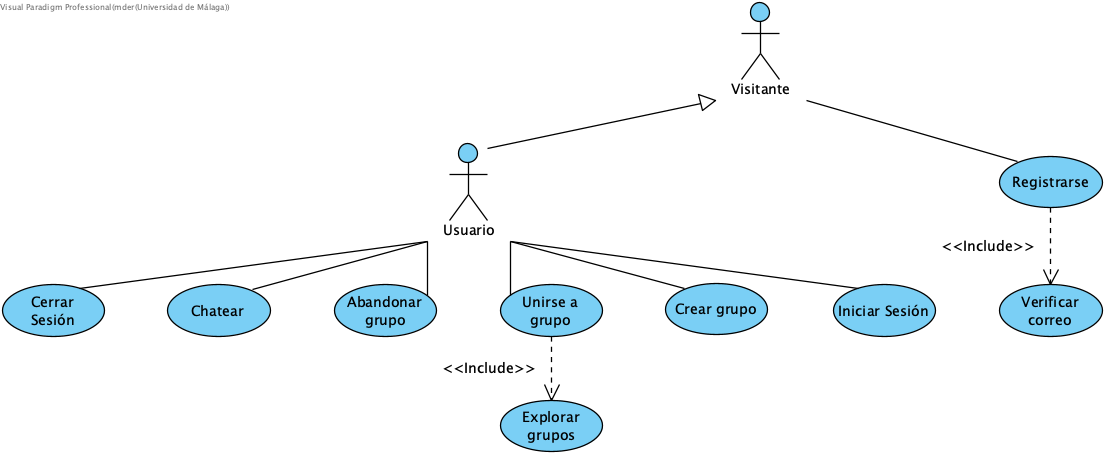
\includegraphics[width=1\linewidth]{images/CasosDeUso.png}
        \caption{Diagrama casos de uso}
        \label{fig:my_label}
    \end{figure}

\subfile{casos/cu01.tex}

\subfile{casos/cu02.tex}

\subfile{casos/cu03.tex}

\subfile{casos/cu04.tex}

\subfile{casos/cu05.tex}

\subfile{casos/cu06.tex}

\subfile{casos/cu07.tex}